\documentclass[tikz,border=8pt]{standalone}
\usepackage{amsmath,amssymb}
\usetikzlibrary{arrows.meta,automata,positioning,quotes}
\begin{document}
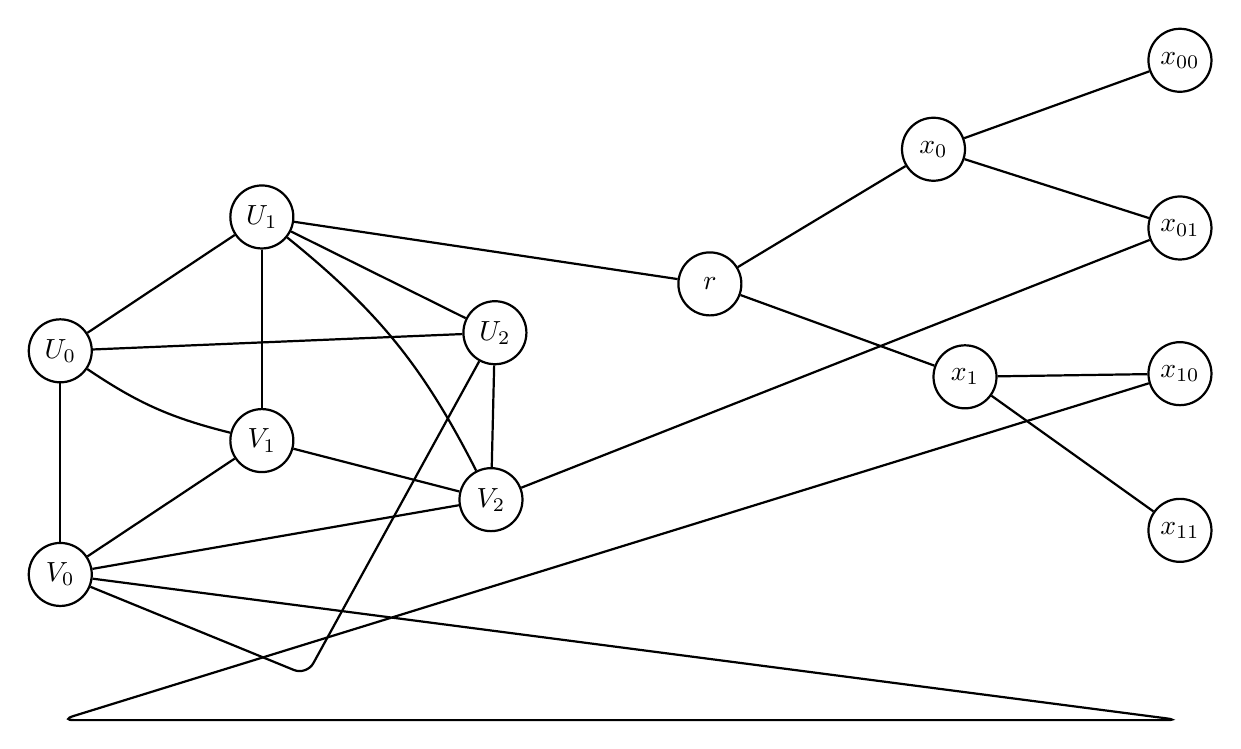
\begin{tikzpicture}[x=1cm,y=1cm]
\tikzset{
  graphnode/.style={circle,draw,thick,minimum size=8mm,inner sep=1pt,font=\sffamily},
  directed/.style={-{Stealth[length=2.4mm]},thick},
  undirected/.style={thick}
}
\node[graphnode] (n_U0) at (-2.37,1.96) {$U_0$};
\node[graphnode] (n_U1) at (0.19,3.66) {$U_1$};
\node[graphnode] (n_U2) at (3.15,2.19) {$U_2$};
\node[graphnode] (n_V0) at (-2.37,-0.88) {$V_0$};
\node[graphnode] (n_V1) at (0.19,0.82) {$V_1$};
\node[graphnode] (n_V2) at (3.10,0.07) {$V_2$};
\node[graphnode] (n_r) at (5.88,2.81) {$r$};
\node[graphnode] (n_x0) at (8.72,4.52) {$x_0$};
\node[graphnode] (n_x1) at (9.12,1.63) {$x_1$};
\node[graphnode] (n_x00) at (11.85,5.65) {$x_{00}$};
\node[graphnode] (n_x01) at (11.85,3.52) {$x_{01}$};
\node[graphnode] (n_x10) at (11.85,1.67) {$x_{10}$};
\node[graphnode] (n_x11) at (11.85,-0.32) {$x_{11}$};
\draw[undirected] (n_U0) -- (n_U1);
\draw[undirected] (n_U1) -- (n_U2);
\draw[undirected] (n_U0) -- (n_U2);
\draw[undirected] (n_V0) -- (n_V1);
\draw[undirected] (n_V1) -- (n_V2);
\draw[undirected] (n_V0) -- (n_V2);
\draw[undirected] (n_U0) -- (n_V0);
\draw[undirected] (n_U1) -- (n_V1);
\draw[undirected] (n_U2) -- (n_V2);
\draw[undirected] (n_U0) to[bend right=10] (n_V1);
\draw[undirected] (n_U1) to[bend left=12] (n_V2);
\draw[undirected,rounded corners=5pt] (n_U2) -- (0.76,-2.16) -- (n_V0);
\draw[undirected] (n_U1) -- (n_r);
\draw[undirected] (n_r) -- (n_x0);
\draw[undirected] (n_r) -- (n_x1);
\draw[undirected] (n_x0) -- (n_x00);
\draw[undirected] (n_x0) -- (n_x01);
\draw[undirected] (n_x1) -- (n_x10);
\draw[undirected] (n_x1) -- (n_x11);
\draw[undirected] (n_x01) -- (n_V2);
\draw[undirected,rounded corners=5pt] (n_x10) -- (-2.37,-2.73) -- (11.85,-2.73) -- (n_V0);
\end{tikzpicture}
\end{document}
